\documentclass[UTF8]{ctexbeamer}
\usetheme{CambridgeUS}
\usecolortheme{lily}

\setbeamertemplate{caption}[numbered]
\usepackage{graphicx}
\usepackage{color}
% \usepackage{times}  

\begin{document}

\title{从DNA序列到系统发育多样性}
\subtitle{进化树的建立和进化相关分析简介}
\author{张金龙}
\institute{嘉道理农场暨植物园}
\date{2019年9月16日} 

\frame{\titlepage} 

\begin{frame}
\frametitle{内容提要}
\begin{itemize}
\item 进化树相关的一些基本概念
\item 建立进化树的基本流程
\item 在R中进行系统发育多样性分析
\end{itemize}
\end{frame}

\begin{frame}
    \frametitle{目录}
    \tableofcontents
    \end{frame}


\begin{frame}
\frametitle{目录}
\section{进化树及相关基本概念}
\tableofcontents[currentsection] 
\end{frame}


\frame{
\frametitle{什么是进化树?}
进化树是表示类群之间系统发育关系的树状结构,是进行系统发育研究(谱系)的基础。
\begin {itemize}
\item cladogram: 体现分类单元甚至个体的{\bf 等级结构},不一定能体现系统发育关系。
\item phylogram: 体现分类单元甚至个体的{\bf 系统发育关系},以精确的枝长反映类群间分化距离。
\item chronogram: 体现分类单元甚至个体的{\bf 系统发育关系},以枝长反映类群间分化的分化时间。
\end {itemize}
}


\frame{
\frametitle{进化树研究的历史}
\begin {itemize}
\item 1837年,达尔文提出了符合进化思想的树状图。\\
\item 十九世纪末,德国人海克尔已经对物种之间的亲缘关系, 建立了基本的进化树。\\
\item 1964年 Cavalli-Sforza 和 Edwards 引入了简约法(parsimony)和似然法(likelihood)。 \\
\item 1966年 Hennig 提出了分支系统学理论(theory of cladistics)。 \\
\item 1977年 Fitch 将简约法应用到DNA序列重建系统发育关系中。 \\
\item 1978年 Felsenstein 最早在计算机中实现了最大似然法,并开发出了PHYLIP软件。\\
\item 1996年 Rannala和杨子恒提出了贝叶斯建树的方法。\\
\end {itemize}
}


\frame{
\frametitle{进化树:树状图}
\begin{center}
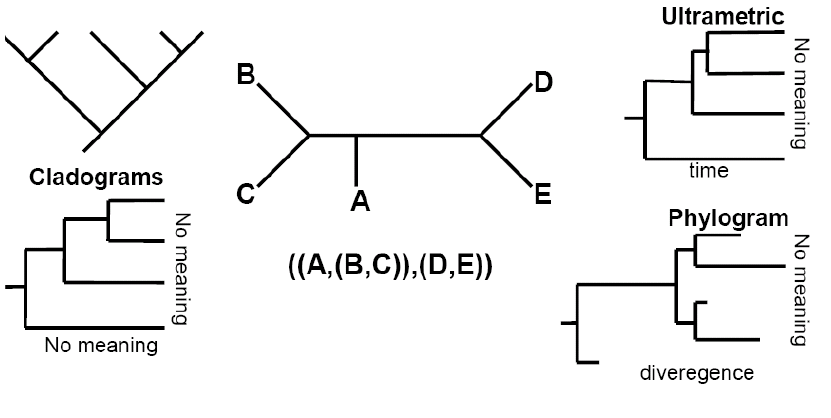
\includegraphics[height=2.1in]{tree.png}\\
\begin{figure}
\caption{各种进化树: 一般从左到右,只计横向枝长。 纵向枝长只是为了图形的美观, 其长度不计。末端节点(tip)一般为物种名称或者个体名称,内部节点(internal nodes)表示分类单元之间的联系}
\end{figure}
\end{center}
}

\begin{frame}[fragile]
\begin{center}
\frametitle{Newick格式}
\begin{figure}
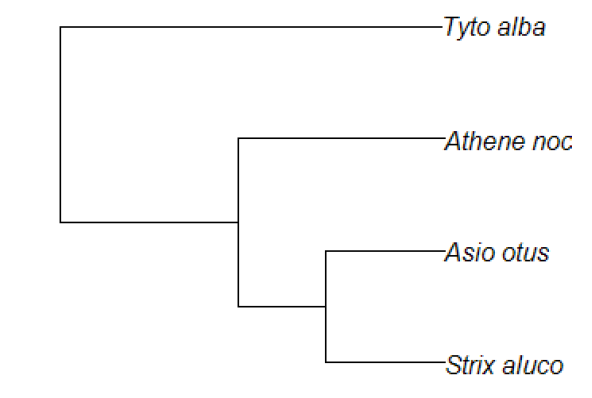
\includegraphics[height=1.4in]{tree2.png}\\
\begin{verbatim}
(((Strix_aluco:4.2, Asio_otus:4.2):3.1, Athene_noctua:7.3):
6.3,Tyto_alba:13.5);
\end{verbatim}
\caption{Newick格式,保存在纯文本文件中:用小括号表示拓扑关系,物种之间用逗号间隔开,物种名后往往添加冒号,冒号后为枝长。冒号前面也可有数字,表示是bootstrap支持率或后验概率等。内部节点可没有名称,而仅有该节点下的枝长。}
\end{figure}
\end{center}


\end{frame}

\begin{frame}[fragile]
\frametitle{NEXUS格式}
\begin{verbatim}
#NEXUS

begin taxa;
dimensions ntax=4; 
taxlabels 
Strix_aluco 
Asio_otus 
Athene_noctua 
Tyto_alba ;
end;

begin trees;
tree tree_1 = (((Strix_aluco:4.2,Asio_otus:4.2):3.1,
Athene_noctua:7.3):6.3,Tyto_alba:13.5);
end; 
\end{verbatim}
\end{frame}

\begin{frame}[fragile]
\frametitle{扩展的Nexus格式、xml格式和Json格式}
\begin{itemize}
\item nexus格式可以进一步包括建树用的DNA序列、定年用的r8s软件、建树用的Paup*命名模块、显示Figtree的模块,MrBayes模块等。
\item xml格式,是一种类似于html的标记语言,用于保存BEAST软件等建树用的数据和相应命令。
\item Json格式(JavaScript Object Notation),是基于JavaScript脚本的一种语言,用于保存DNA序列和某些软件的命令。
\end{itemize}

余光创博士编写的ggtree程序包提供了多种格式的读取和简单处理。

\end{frame}


\frame{
\frametitle{进化树的编辑和打印}
以下软件,提供了编辑Newick文件或者Nexus文件的功能。 
\begin {itemize}
\item Mesquite:用Java开发,有众多插件,能进行DNA序列、进化树、性状的编辑并多种系统发育比较分析。
\item FigTree:用JAVA编写,无需安装,对Newick和Nexus支持很好,参数较多, 容易调整, 跨平台。
\item TreeView:早期查看进化树的经典软件,但是参数不好控制。 
\item MEGA:一般针对该软件自己生成的进化树绘图等,支持Newick树的可视化编辑。
\item Dendroscope: 对Newick格式和Nexus支持较好,类似FigTree,同时支持Singletons。
\item iTOL:网页版,编辑进化树
\end{itemize}
}

\frame{
\frametitle{进化树出图用的R包}

\begin {itemize}
\item ape: 由E. Paradis等编写,其内置的plot.phylo函数,功能灵活,拥有绘制进化树的多种参数。
\item ggtree: 由余光创博士开发,支持ggplot2的语法。支持多种数据格式的读写。
\end{itemize}
}


\frame{
\frametitle{建立进化树的前提:基因的同源性}
\begin {itemize}
\item ortholog: 这个基因出现在所有的后代物种中,由共同祖先的同一个基因演变而来。\\
\item paralog: 该基因出现在一个体内, 由共同祖先基因扩增而来 \\
\item xenolog: 基因转座\\
\end{itemize}
进化树推断中, 必须要用orthological同源基因\\
}

\frame{
\frametitle{等距树、有根树和外类群及其选择}
\begin {itemize}
\item 等距树(Ultrametric Tree):进化树中, 每一个末端分类单元都与根节点的距离相等.\\
\item 有根树(rooted tree)和无根树(unrooted tree):为了探讨一个类群内部的亲缘关系,需要在进化树中指定一个或几个独立于所研究类群之外的分类单元作为外类群(outgroup)。指定了外类群的树,称为有根树,否则称为无根树。有根树能够表示类群内部的亲缘关系,而无根树只能显示拓扑结构。 \\
\item 外类群: 通常选择研究类群的近缘的单系类群作为外类群,不能位于研究类群中,也不能距离所研究的类群太远。前者无法体现类群的进化关系,后者在序列比对,或者进化树推断时会造成结果不准确。\\
\end{itemize}
}

\begin{frame}
\frametitle{无根树 Unrooted Tree}

\begin{center}
\begin{figure}
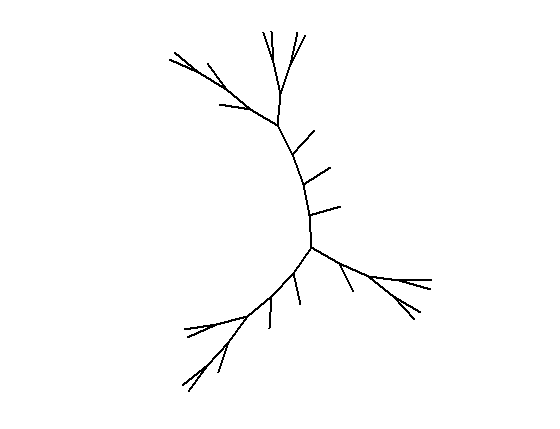
\includegraphics[height=2.2in]{unrooted.png}\\
从哪里开始?到哪里结束?\\
\caption{无根树。在建树时没有指定外类群,则进化树为无根树,在后续操作时,首先应转换为有根树(rooted tree)}
\end{figure}
\end{center}
\end{frame}


\begin{frame}
\frametitle{外类群的指定}
\begin{center}
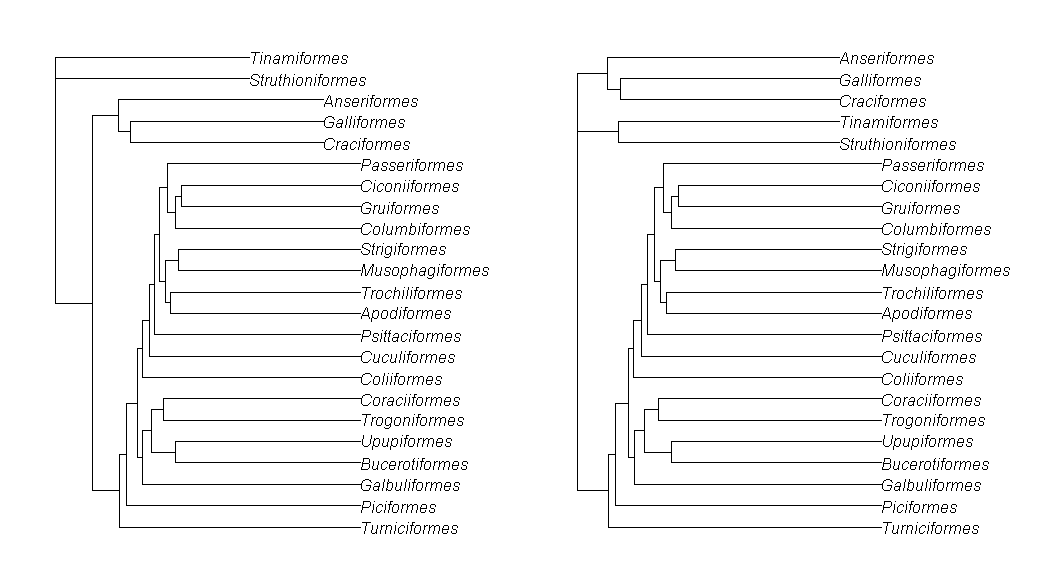
\includegraphics[height=2.3in]{rooted.png}\\
\end{center}

\begin{figure}
\caption{外类群的数量,可以根据研究需要进行指定。用Figtree和ape指定外类群十分方便。}
\end{figure}

\end{frame}

\begin{frame}
\frametitle{一致性树 Consensus Tree}
\begin{itemize}
\item 当获得了多个拓扑结构时,需要对拓扑结构的稳定性,即进化树内部的各节点的可靠性进行判断。\\
\item 对进化树内部的节点,进行可靠性检验后,常常会生成大量进化树,需要对结果进行汇总。\\
\item 按照节点一致性原则,选出各进化树都支持的某节点的拓扑结构,并计算支持该节点的百分率,就称为支持率。 \\
\item 支持率低的节点, 有时候选择合并,这样就形成了多分枝结构(Polytomies)
\end{itemize}
\end{frame}

\begin{frame}
\frametitle{多分枝结构}
\begin{center}
\begin{figure}
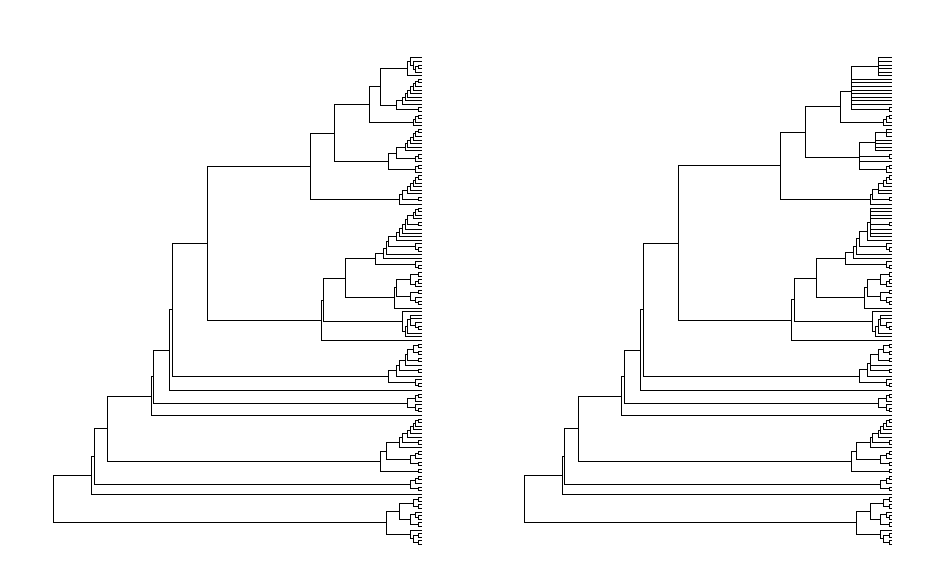
\includegraphics[height=2.6in]{polytomies.png}\\
\caption{多分枝结构}
\end{figure}
\end{center}
\end{frame}

\begin{frame}
\frametitle{多分枝结构的成因}
若某一个节点支持率很低, 表明现有数据不能将该节点下的各分类单元分开\\
多分枝结构的成因: \\
\begin{itemize}
\item 数据缺失, 或所选的建树基因变异很低,无法体现足够的系统发育信息。\\ 
\item 物种的快速辐射进化,如环境对表型的强烈筛选,近缘种在短时间内形成了多个物种。这些亲缘种之间,用某一基因常常难以区分。\\
\end{itemize}
\end{frame}


\begin{frame}
\frametitle{二叉树和孤立节点}
\begin {itemize}
\item 一般情况下, 每个节点下, 应该直接分成两个姊妹节点,这种进化树称为二歧树(divaricate),也称二叉树。\\
\item 若一个节点下, 只有一个节点, 则称其为孤立节点(Singleton)。
\item 群落系统发育分析的Phylomatic软件在建立进化树时,会生成很多多分枝结构和孤立节点。Phylocom软件则能处理含有孤立节点的newick进化树\\
\item 若进化树含有多分枝结构,而数据分析软件要求输入二叉树,则可使用ape包的multi2di函数转换,为多分枝结构的节点,随机添加一个很小的枝长,从而转换为二叉树。
\end{itemize}
\end{frame}


\frame{
\frametitle{FASTA文件}
\begin {itemize}
\item FASTA文件为纯文本格式。
\item 物种的DNA序列常以该文件格式保存。
\item 每条序列以$>$开头。
\item 换行后为该条核苷酸序列 'ATCG'
\item FASTA文件也可以保存比对后的序列。
\item FASTA数据与换行(interleaved)和不换行的区别。
\end{itemize}
}


\begin{frame}
\frametitle{FASTA文件示意图}
\begin{center}
\begin{figure}
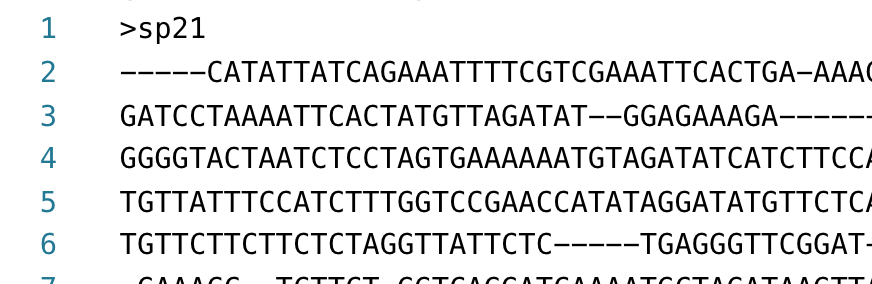
\includegraphics[height=1.2in]{fasta_example.png}\\
\caption{FASTA文件}
\end{figure}
\end{center}
\end{frame}


\section{DNA序列的获取和比对}

\frame{
\frametitle{DNA序列的获取}
DNA数据,按照来源可分成三类:\\
\begin {itemize}
\item 测序数据,包含桑格(一代)测序,高通量(二代、三代)测序,单分子测序等。
\item 从数据库下载,GenBank、EBI、DDBJ等综合数据库,以及各类专业数据库。
\item 模拟数据:用软件按照一定规则,随机生成的数据
\end{itemize}
DNA条形码,就是一种快速获取DNA序列的方法。
}


\frame{
\frametitle{DNA条形码建立进化树的基本技术流程}
\begin {itemize}
\item 采样:注意一定要有凭证标本
\item 总DNA提取和琼脂糖电泳检测
\item 目的序列的PCR和琼脂糖电泳检测
\item 送公司测序,获得ab1峰图文件和fasta文件,测序质量检查(ChromasPro软件等),正反测序结果合并和校对(如DNAman软件,ContigExpress软件,VectorNTI等)
\item 通过和BLAST数据库比对,检查是否存在污染和测序错误,确认和保存为Fasta文件
\item 用MUSCLE比对,进一步检查,在BioEdit或者AliView中检查
\item 每个基因,分别建树检查各分类单元的系统发育关系。用多个基因,建立Supermatrix检查
\end{itemize}
}


\frame{
\frametitle{序列比对}
目的:将具有变异信息的位点对齐\\
\begin {itemize}
\item ClustalX:图形用户界面,但是比对速度较慢 (过去主流)
\item MUSCLE:命令行,适用于较大大规模数据 (当前主流)
\item Mafft:命令行,能处理30000条以内的DNA序列比对(当前主流)
\item PRANK:DNA和氨基酸序列的比对(当前主流)
\item TranslatorX, MASCE:主要用于编码区的比对
\end{itemize}
}


\frame{
\frametitle{比对前的DNA序列}
\begin{center}
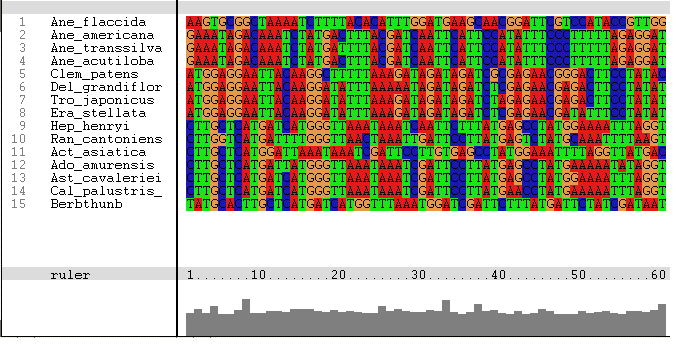
\includegraphics[height=2in]{Aligment1.png}\\
\begin{figure}
\caption{比对前的序列}
\end{figure}
\end{center}
}

\frame{
\frametitle{比对后的DNA序列}
 \begin{center}
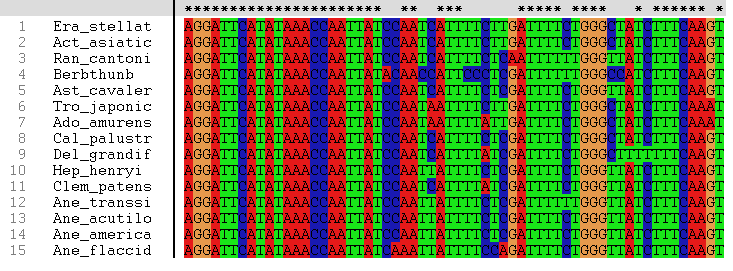
\includegraphics[height=1.5in]{Aligment2.png}\\
\begin{figure}
\caption{比对后的序列}
\end{figure}

\end{center}
}

\frame{
\frametitle{比对后的手工校正}
测序的错误,可能在比对后才能体现出来,因此需要核对测序的荧光染料强度峰图,进行人工判读和修改。\\
对于编码基因,三联体密码子,缺失的位置和长度必须是3的倍数\\
软件: 
\begin {itemize}
\item AliView 较新,跨平台
\item BioEdit 传统,仅Windows
\item Geneious 功能强大的集成分析软件
\end{itemize}
}

\frame{
\frametitle{BioEdit}
 \begin{center}
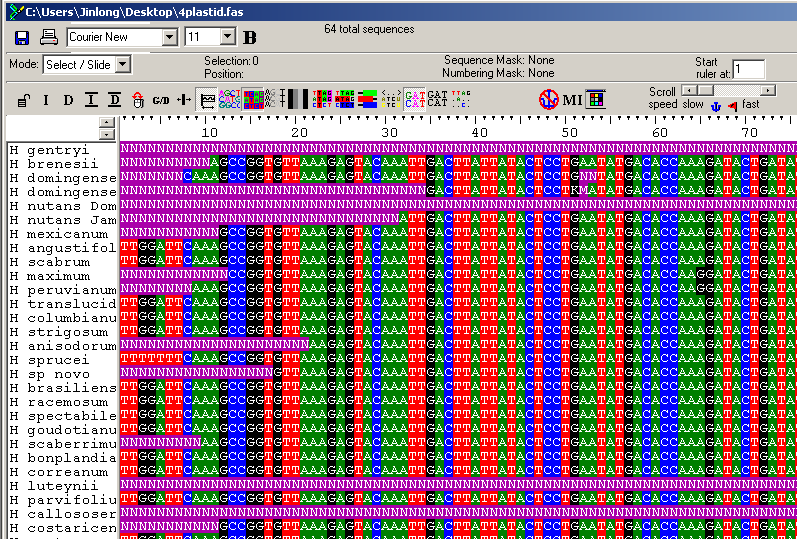
\includegraphics[height=2.5in]{BioEdit.png}\\
\begin{figure}
\caption{用Bioedit编辑序列}
\end{figure}
\end{center}
}


\begin{frame}
\frametitle{目录}
\section{进化模型及其筛选}
\tableofcontents[currentsection] 
\end{frame}


\frame{
\frametitle{进化模型}
A \: A$\rightarrow$  A\: A $\rightarrow$  G\: G$\rightarrow$ T 

\[Prob[k\, events]=\frac{(\mu t)^{k}e^{-\mu t}}{k!}\]

符合统计学中的泊松分布(Poisson Distribution)\\
$\mu$ 为碱基替换率

$R_{xy}$ 为位点从x, 转变为y, 的概率。

\[Prob(t)=\sum_{k=0}^{\infty}\text{(}R^{k})\frac{(\mu t)^{k}e^{-\mu t}}{k!}\]
 
\[Prob(t)=\sum_{k=0}^{\infty}\frac{(R-1)^{k}(\mu t)^{k}}{k!}=\sum_{k=0}^{\infty}\frac{(Q\mu t)^{k}}{k!}=e^{Q\mu t}\]
}

\frame{
\frametitle{进化模型}
\[ Q=\left[\begin{array}{cccc}
- & r_{AC} & r_{AG} & r_{AT}\\
r_{CA} & - & r_{CG} & r_{CT}\\
r_{GA} & r_{GC} & - & r_{GT}\\
r_{TA} & r_{TC} & r_{TG} & -
\end{array}\right]\]

行表示初始状态, 列表示转变后的状态。

\[q_{ii}=-\sum_{j=0,j\neq i}^{4}q_{ij}\]
 
Q为转移概率矩阵
}

\frame{
\frametitle{转移概率矩阵模型 JC69模型}
由 Jukes and Cantor (1969) 提出。\\
转移概率矩阵模型\\
{\tiny \[Q=\left[\begin{array}{cccc}
-\mu(a\pi_{C}+b\pi_{G}+c\pi_{T}) & a\mu\pi_{C} & b\mu\pi_{G} & c\mu\pi_{T}\\
g\mu\pi_{A} & -\mu(g\pi_{A}+d\pi_{G}+e\pi_{T}) & d\mu\pi_{G} & e\mu\pi_{T}\\
h\mu\pi_{A} & i\mu\pi_{C} & -\mu(h\pi_{A}+j\pi_{C}+f\pi_{T}) & f\mu\pi_{T}\\
j\mu\pi_{A} & k\mu\pi_{C} & l\mu\pi_{G} & -\mu(i\pi_{A}+k\pi_{C}+l\pi_{G})
\end{array}\right]\]}\\

JC69模型\\
\[Q=\left[\begin{array}{cccc}
- & 1 & 1 & 1\\
1 & - & 1 & 1\\
1 & 1 & - & 1\\
1 & 1 & 1 & -
\end{array}\right]\]

参考:?dist.dna
 }

\frame{
\frametitle{转移概率矩阵模型 Kimura 81 和 F81}
Kimura 81: 考虑transition或transversion\\
例如由G变成A 称为transition\\
A转变成T,或T变成A, 称为transerversion。\\
\[ Q=\left[\begin{array}{cccc}
- & 1 & \text{\ensuremath{\kappa}} & 1\\
1 & - & 1 & \kappa\\
\kappa & 1 & - & 1\\
1 & \kappa & 1 & -
\end{array}\right] \]

F81 (Felsenstein, 1981)\\
\[ Q=\left[\begin{array}{cccc}
- & \pi_{C} & \pi_{G} & \pi_{T}\\
\pi_{A} & - & \pi_{G} & \pi_{T}\\
\pi_{A} & \pi_{C} & - & \pi_{T}\\
\pi_{A} & \pi_{C} & \pi_{G} & -
\end{array}\right]\]

$\pi_{i}$
 is the equilibrium frequency of nucleotide i\\

}

\frame{
\frametitle{转移概率矩阵模型 F84}

F84 (Felsenstein, 1984)\\
\[Q=\left[\begin{array}{cccc}
- & \pi_{C} & (1+\kappa/\pi_{R})\pi_{G} & \pi_{T}\\
\pi_{A} & - & \pi_{G} & (1+\kappa/\pi_{Y})\pi_{T}\\
(1+\kappa/\pi_{R})\pi_{A} & \pi_{C} & - & \pi_{T}\\
\pi_{A} & (1+\kappa/\pi_{Y})\pi_{C} & \pi_{G} & -
\end{array}\right]\]
 
$\pi_{i}$
 : the equalibrium frequency of nucleotide i\\
$\kappa=\alpha/\beta$
 
$\alpha$
 : transition matrix\\
$\beta$
 : the transversion rate\\

}

\frame{
\frametitle{更多转移概率矩阵模型二}
HKY85 (Hasegawa-Kishino-Yano, 1985)\\
\[ Q=\left[\begin{array}{cccc}
- & \pi_{C} & \kappa\pi_{G} & \pi_{T}\\
\pi_{A} & - & \pi_{G} & \kappa\pi_{T}\\
\kappa\pi_{A} & \pi_{C} & - & \pi_{T}\\
\pi_{A} & \kappa\pi_{C} & \pi_{G} & -
\end{array}\right] \]
 
Tamura-Nei, 1993\\
\[ Q=\left[\begin{array}{cccc}
- & \pi_{C} & \kappa_{2}\pi_{G} & \pi_{T}\\
\pi_{A} & - & \pi_{G} & \kappa_{1}\pi_{T}\\
\kappa_{2}\pi_{A} & \pi_{C} & - & \pi_{T}\\
\pi_{A} & \kappa_{1}\pi_{C} & \pi_{G} & -
\end{array}\right] \]

 
\text{其中} $\kappa_{1}=\alpha_{Y}/\beta\text{,}$
 $\kappa_{2}=\alpha_{R}/\beta$
 
$\alpha_{R}\text{:}$
 the purine transition rate
$\alpha_{Y}$
 :the pyrimidine transition rate 
$\beta$
 :the transversion rate
}


\frame{
\frametitle{统一模型GTR}
General Time Reversible Model\\
\[Q=\left[\begin{array}{cccc}
- & \alpha\pi_{C} & \beta\pi_{G} & \gamma\pi_{T}\\
\text{\ensuremath{\alpha}}\pi_{A} & - & \delta\pi_{G} & \epsilon\pi_{T}\\
\beta\pi_{A} & \delta\pi_{C} & - & \eta\pi_{T}\\
\gamma\pi_{A} & \epsilon\pi_{C} & \eta\pi_{G} & -
\end{array}\right]\]

$\alpha$$...$$\eta$
 :从一种碱基变换为另一种碱基的速率
$\pi$
 碱基频率
将参数$\alpha...\eta$
  做一定的限制,GTR模型可以简化为以上任何一种转移概率模型
 
 }

\frame{
\frametitle{模型之间的关系}
\begin{center}
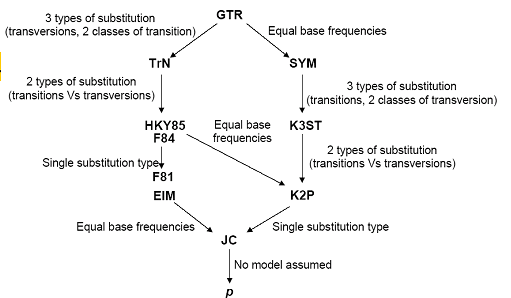
\includegraphics[height=2.5in]{models.png}\\
\begin{figure}
\caption{DNA碱基替换模型间的关系}
\end{figure}
\end{center}
}

\frame{
\frametitle{碱基位点变异速率的差异}
密码子的第三个碱基比前两个碱基变异更快;\\
不同区域的功能不同, 变异速率存在差异。\\
为此,人们引入Gamma分布拟合不同位点进化速率的差异.
\[\Gamma(a)=\int_{0}^{\infty}x^{a}e^{-x}\frac{dx}{x},\; a>0\]
}


\frame{
\frametitle{碱基替换模型的筛选}
什么样的模型是合适的?\\
对于巢式模型(nested models)的筛选,采用似然比检验(Hierarchical Likelihood Ratio Test)\\
即:求每个进化树的最大似然值,即给定进化模型M,模型的各参数$\theta$\\
进化树拓扑结构$\tau$以及枝长 $\nu$当前序列比对格局出现的概率。\\
 
\[L=P(D\mid M,\theta,\tau,\nu)\]\\
 
为了使该序列比对格局出现的可能性最大,对Likelihood function取最大值\\
\[ \hat{\theta},\hat{\tau},\hat{\nu}=\mathrm{max}L(\theta,\tau,\nu) \]\\
}
 
\frame{
\frametitle{碱基替换模型的筛选}
取对数
\[ \ell=\mathrm{ln}P(D|M,\hat{\theta},\hat{\tau},\hat{\mu})\]
 
\[LRT=2(\ell_{1}-\ell_{2})\]
 
$LRT(Log Likelihood Ratio)$ , 符合 $\chi^2$分布。因此可检验模型复杂程度的变化是否对模型的精度有显著的影响。\\

赤池信息量 AIC(Akaike Information Criterion)\\
一般作为模型的准确性(Likelihood部分)和参数数量(k)之间的权衡。\\
\[AIC=-2\ell+2k\]

软件: ModelTest、jModelTest、PartitionFinder、IQ-TREE等\\
}

\begin{frame}
\frametitle{目录}
\section{建立进化树的方法}
\tableofcontents[currentsection] 
\end{frame}


\frame{
\frametitle{构建进化树的主要方法 I}
碱基概率转移模型保证我们获得建立进化树所需的枝长,但是如何获得进化树的拓扑结构?\\
\begin {itemize}
\item 1.距离法 (Distance based method):根据序列两两之间的进化距离,进行聚类\\
\item 2. 简约法 (Most Parsimony):根据序列之间变化的关系, 找到一棵树, 使该进化树上所发生的进化事件(碱基替换发生的次数)最少。\\

\end{itemize}
}

\frame{
\frametitle{构建进化树的主要方法 II}
\begin {itemize}
\item 3.极大似然法 (Maximum Likelihood):在所有拓扑结构中找出最有可能形成当前序列比对格局的拓扑结构。\\
\item 4.贝叶斯法 (Bayesian):从一系列可能取值中, 随机给出参数的初始值,让进化树的参数在参数空间按照后验概率密度移动, 生成成千上万棵进化树,对这些进化树进行信息汇总, 从而得到进化树拓扑结构和枝长分布的估计。\\

\end{itemize}
}

%%%%%%%%%%%%%%%%%%%%%%%%%% 20190907 更新到此处 %%%%%%%%%%%%%%%%%%%%%%%%%%

\frame{
\frametitle{进化树建立:遗传距离法}
{\bf 第一步}:计算序列之间的遗传距离矩阵\\
遗传距离可以基于RAW,即碱基差异的数量,或者Transition,transversion,也可以基于各种转移概率模型。计算可参考ape软件的dist.dna()\\
{\bf 第二步}:基于距离矩阵进行聚类\\
\begin{itemize}
\item UPGMA法(Unweighted Pair Group Method with Arithmetric Mean)\\
\item NJ法: Neighbour Joining\\
\item ME法: 最少进化法 Minimum Evolution\\
\end{itemize}
目前,由NJ法或ME法创建的进化树,一般只用于构建极大似然进化树的初始树,极少能再作为论文的最终结果。
}

\frame{
\frametitle{进化树建立:最大简约法}
进化速率低的序列, 回复突变很少,此时可以用最大简约法。

{\bf 简约原理}\\
真实的进化历史的经历的进化事件最少。\\

优点:\\
\begin {itemize}
\item 结果容易解释\\
\item 计算速度快\\
\item 进化树结构良好\\
\end {itemize}

什么时候用简约法建树?\\
\begin {itemize}
\item 作为其它方法的初始进化树\\
\item 基因家族进化历史的推断\\
\end {itemize}
PAUP*适用于建立最大简约树\\
}


\frame{
\frametitle{进化树建立:最大似然法}
最大似然估计一种参数估计的方法。按照当前的概率,数据所出现概率的乘积称为似然(Likelihood)。
\[L(H)=\prod Prob(D|H)=Prob(D_{1}|H)Prob(D_{2}|H)\cdot\cdot\cdot Prob(D_{n}|H)\]
 
\[Prob[D_{j}|\tau,M,\rho_{j},],\; j=1,2,...n\]
 
\[L(\tau,M,\rho|D)\equiv Prob[D|\tau,M,\rho]=\prod_{j=1}^{l}Prob[D_{j}|\tau,M,\rho_{j}]\]
 
因此,Likelihood为联合概率密度,当所有发生某一事件的概率密度(假设的概率密度)相乘,其结果取最大值时,就发生了当前的事件,这就是极大似然的思想。\\ 


应用于进化树推断时,问题变为:{\bf 假设已经有一棵进化树T以及碱基替换模型Q,则获得当前DNA比对格局的可能性有多大?}
}

\frame{
\frametitle{进化树建立:最大似然法}
\[L(T, Q) = Prob(D|T, Q)\]一些常用假设:\\
\begin {itemize} 
\item 不同位点的进化彼此独立\\
\item 不同分支的进化彼此独立\\
\item 各位点的进化速率相同\\
\end {itemize}
\[L(\tau,M,\rho|D)\equiv Prob[D|\tau,M,\rho]=\prod_{j=1}^{l}Prob[D_{j}|\tau,M,\rho_{j})\]
 
给定进化树,比对格局的总体似然值无法直接用表达式计算,进化树内部的每个节点与两个子代之间似然函数的关系为:
\[L_{j}^{i}(s)=\left[\sum_{x\in\{A,C,G,T\}}P_{sx}(d_{o1})L_{j}^{o1}(x)\right]\centerdot\left[\sum_{x\in\{A,C,G,T\}}P_{sx}(d_{o2})L_{j}^{o2}(x)\right]\]
 }
 
\frame{
\frametitle{进化树建立:计算Likelihood}
对于末端节点, 如果 $s=s_{i}^{j}$
 ,则\[L_{j}^{i}(s)=1\]否则
 \[L_{j}^{i}(s)=0\]
 
 \[Prob[D_{j},\tau,Q,1]=\sum_{s\in{A,C,G,T}}\pi_{s}L_{j}^{2n-2}(s)\]
 
此时整个碱基比对格局的似然值为:\[log[L(\tau,M,1)]=log\left[\prod_{j=1}^{l}Prob[D_{j,}\tau,Q,1]\right]
=\sum_{j=1}^{l}log\left[Prob[D_{j},\tau,Q,1]\right] \]
 

}
\frame{
\frametitle{计算机是如何计算极大似然法进化树的?}
\begin {itemize} 
\item 对一系列参数给出随机值或基于简约法计算出的数值,作为初始值。\\
\item 每次对之前所得的参数数值做一定程度的改变, 每次计算LogLikelihood,直到LogLikelihood不再改变为止。\\
\item 所得参数就是进化树的极大似然估计。\\
\end {itemize} 

哪些参数需要改变?\\
\begin {itemize} 
\item 1. 进化树的拓扑结构和枝长\\
\item 2. 碱基替换之间的转移概率矩阵Q\\
\item 3. 不同区段的碱基替换频率的差异(Gamma distribution)\\
\end {itemize} 
}

\begin{frame}
    \frametitle{目录}
    \section{启发式搜索和bootstrap可靠性评估}
    \tableofcontents[currentsection] 
    \end{frame}

\frame{
\frametitle{进化树的数量}
需要在多少种拓扑结构中搜寻?\\
答: 随着进化树中物种数的增加,进化树的拓扑结构数量迅速增加。\\
每新增加一个分类单元, 都能够在之前的2n-3个位置放置进化树\\
进化树的数量, 因此, 进化树的数量与分类单元的数量的关系为: \\
\[ t_{n}=\frac{(2n-5)!}{2^{n-3}(n-3)!}=\prod_{i=1}^{n}(2i-5) \]

}

\frame{
\frametitle{进化树的数量}
{\tt 3: 1 \\
4: 3 \\
5: 15 \\
6: 105 \\
7: 945 \\
8: 10,395 \\
9: 135,135 \\
10: 2,027,025 \\
11: 34,459,425 \\
12: 654,729,075 \\
13: 13,749,310,575 \\
14: 316,234,143,225 \\
15: 7,905,853,580,625 \\

}
}

\frame{
\frametitle{进化树的数量}
{\tt 16: 213,458,046,676,875 \\
17: 6,190,283,353,629,374 \\
18: 191,898,783,962,510,624 \\
19: 6,332,659,870,762,850,304\\
20: 2.216430954767e+20\\
30: 8.687364e+36 \\
50: 2.838063e+74\\
{\bf Bang!!!}\\
}
通常,在所有的拓扑结构中搜索是不可能的\\
因此在分类单元数较多时,需要用到启发式搜索(heuristic search).
}

\frame{
\frametitle{启发式搜索: 物种逐步添加}
以一棵随机的、只包含三个种的进化树开始,在剩余数据中,随机找出一个物种,加入到进化树中。随着加入位置的不同,所得的比对格局的Likelihood不同,取能够使Likelihood最高的加入位置,继续加入剩余的节点,直到所有物种加入到进化树中。这种添加物种的方式,称为{\bf 物种逐步添加 (stepwise addition)},是一种启发式搜索。\\
}

\frame{
\frametitle{减少局域最大似然的影响}
但是对于n个物种的进化树来说,我们只计算了$(n-2)^{2}$\\个进化树,所得的极大似然值,并不一定为所有可能的进化树中最大的,因此,结果很可能为{\bf 局域最大似然值(regional maximum likelihood)}。\\
为了尽量减少局域最大似然的影响,生物信息学家采用以下方法:\\
\begin{itemize}
\item 1. 多次从随机的进化树开始,随机添加物种\\
\item 2. 进化树的剪接和重排\\
\item 3. 对于接近最优树的进化树进行重排,以便寻找全局最优树\\
\end{itemize}
}

\frame{
\frametitle{进化树的重排}
进化树重排,是对现有进化树的分支结构进行剪接后, 再按照一定规则连接起来的一系列方法,包括\\
\begin{itemize}
\item NNI: Nearest neibourgh interchange $2(n-3)$\\
\item SPR: sub-tree pruning and regrafting $4(n-3)(n-2)$\\
\item TBR: tree bisection and reconstruction $(2n_{1}-3)(2n_{2}-3)$\\
\end{itemize}

TBR是最复杂的进化树剪接方式,NNI和SPR都可以看做TBR的特例。
}

\frame{
\frametitle{进化树重排}
\begin{center}
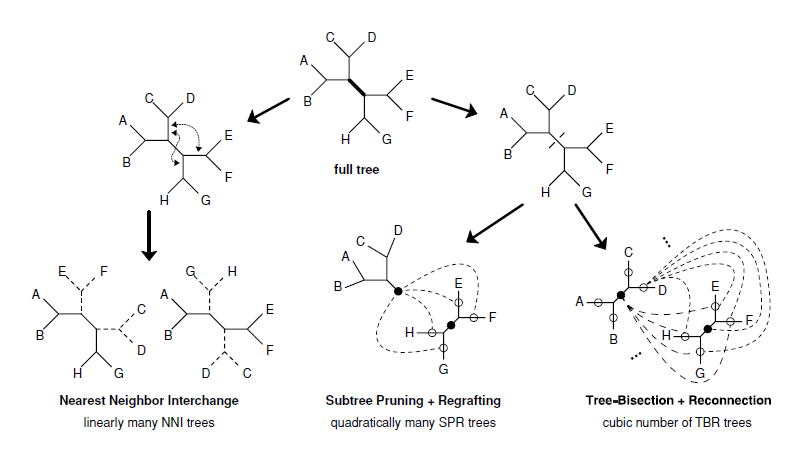
\includegraphics[height=2.5in]{TBR.png}\\
\begin{figure}
\caption{进化树重排的方法:NNI,SPR和TBR}
\end{figure}
\end{center}
}


\frame{
\frametitle{启发式搜索中的问题}
启发式搜索, 只保留每一步的最优树,作为下一步的起始值。在进化树的空间中,进化树可能最终到达局部最优,而无法达到全局最优。

为了进一步接近全局最优, 人们开发了多种方法:
\begin{itemize}
\item 进化树合并(tree-fusing)
\item 遗传算法(genetic algorithms)
\item 进化树局部全搜索(tree windowing)
\item 加权搜索(search by reweighting)
\item 模拟退火(simulated annealing)
\end{itemize} 
}

\frame{
\frametitle{贪婪算法可靠吗?}
\begin{center}
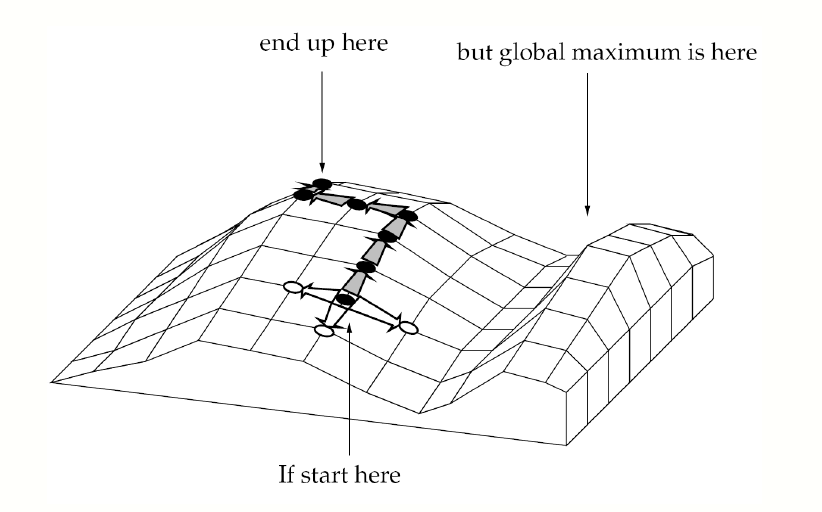
\includegraphics[height=2.5in]{greedyAlgorithm.png}\\
\begin{figure}
\caption{贪婪算法为什么容易找到局域最优进化树?}
\end{figure}
\end{center}
}




\frame{
\frametitle{进化树可信度评估Bootstrap}
已知样本数据, 如何求某一统计量在总体中的分布? \\
Bootstrap是利用样本数据进行可放回的抽样, 形成大量Boostrap拟样本后, 每个样本进行和源数据相同的分析,从而得到某一统计量的分布。\\
如:从Boostrap的1000个bootstrap样本可获得1000棵进化树,对这1000棵进化树和真实数据形成的进化树进行比较, 即可获得每个节点的支持率。
}


\frame{
\frametitle{进化树的Bootstrap支持率}
\begin{center}
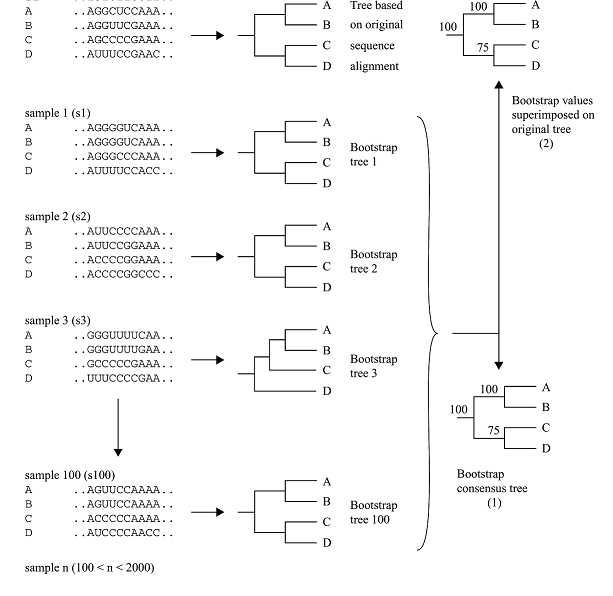
\includegraphics[height=2.6in]{Bootstrap.png}\\
\begin{figure}
\caption{进化树可靠性的Bootstrap检验}
\end{figure}
\end{center}
}


\frame{
\frametitle{Maximum Likelihood建树软件 I:往日的辉煌}
\begin{itemize}
\item PHYLIP: 由美国Joe Felsenstein编写,开源软件,也是第一个用极大似然法搜索进化树的软件,适用于进化树入门学习和小规模数据的进化树建立\\
\item PAUP*: 由美国David Swoford编写,特别适用于最大简约法,但是也包括极大似然法以及各种搜索以及进化树剪接,Bootstrap等。还可以结合ModelTest进行进化模型筛选。但是需要购买版权。\\
\end{itemize}
}


\frame{
\frametitle{Maximum Likelihood建树软件 II:当今的王者}
\begin{itemize}
\item PHYML:由法国的Guidon编写,适用于大规模数据(大量分类单元或大量信息位点)。支持多种模型的筛选。\\
\item RAxML:由瑞士Stamatakis编写只支持DNA的GTR模型以及蛋白质的模型,适用于分类单元数较多,或者位点数较多时,建立极大似然进化树,运用快速bootstrap,甚至可以基于整个基因组建立进化树。\\
\item IQTREE:软件较新,由越南的Bui Quang Minh等开发。支持模型筛选、快速bootstrap。效率和准确度甚至高于RAxML,目前是建立进化树的最佳选择之一。
\end{itemize}
}

\begin{frame}
    \frametitle{目录}
    \section{贝叶斯法建树}
    \tableofcontents[currentsection] 
    \end{frame}

\frame{
\frametitle{频率学派}
频率学派:给定当前的假设,观察到当前的样本的概率是多少?\\
求P值\\
通过样本数据,根据某一假设的统计分布假设,计算出的统计量,在统计量的分布中,出现在哪个区间,从而求得P值。\\
\begin{itemize}
\item 1 被估计的参数未知,但是有一个确定值。\\
\item 2 需要根据重复取样对概率分布进行客观取样\\
\item 3 样本量越大,参数的估计就越准确\\
\item 4 进行极大似然估计\\
\end{itemize}
}

\frame{
\frametitle{贝叶斯学派}
贝叶斯推断是参数估计的一种方法,但是贝叶斯推断不是估计出参数的固定值, 而是生成估计对象的分布。\\
贝叶斯学派:给定样本数据,待估计参数的概率分布如何?\\
主要特征:\\
1 待估计的参数是统计分布\\
2 主观得假设参数服从某种分布(先验分布)\\
3 无需大样本\\
4 基于统计模拟,对参数进行估计\\
}


\frame{
\frametitle{贝叶斯法则}
\[p(\theta|y)=\frac{p(y|\theta)p(\theta)}{p(y)}\]
 
$\theta$
 是待估计的参数
$y$
 是样本数据
$p(y|\theta)$
 是样本的概率密度(Likelihood)
$p(\theta)$
 是主观假定的参数概率密度
$p(y)$
 是 Normalizing constant
\[p(y)=\int P(y|\theta)P(\theta)d\theta\]
 即所有生成当前数据的概率相乘。很多情况下,$p(y)$
 是无法用表达式求出的。而是要用到MCMCMC的方法。
}


\frame{
\frametitle{贝叶斯方法的优缺点}
优点\\
\begin{itemize}
\item 能够计算出待估计参数的概率分布\\
\item 能够解决常规方法不能解决的复杂问题\\
\end{itemize}
缺点\\
\begin{itemize}
\item 需要高深的统计知识\\
\item 需要强大的计算能力\\
\item 在指定参数的先验概率分布时,需要进行足够的解释\\
\end{itemize}
一般用蒙特卡洛马尔科夫链 Metropolis coupling(Monte Carlo Markov Chain Metropolis Coupling, MCMCMC, $MC^3$)的方法生成参数的分布, 但是结果是否收敛, 没有很好的评判标准。\\
}


\frame{
\frametitle{蒙特卡罗马尔科夫链 Metropolis coupling (MCMCMC)}
\[p(y)=\int P(y|\theta)P(\theta)d\theta \]
 贝叶斯积分一般难以获得解析解。在无法获得参数联合概率密度的情况下,蒙特卡罗马尔科夫链可以保证人们在后验分布的参数空间中取样,当获得大量后验分布的样本后, 即可获得后验概率的近似分布。\\
{\bf 事件的马尔科夫性:} 某一事件在t时刻状态B的概率只与之前一个时刻$t_{0}$的状态A有关,而与$t_{0}$时刻之前的状态以及t之后的状态无关。\\
对于进化树\\
\[prob(Tree,\theta|Sequence)=\frac{prob(Tree,\theta)prob(Sequence|Tree,\theta)}{prob(Sequence)}\]\\

}

\frame{
\frametitle{构建进化树思路的比较}
\begin{center}
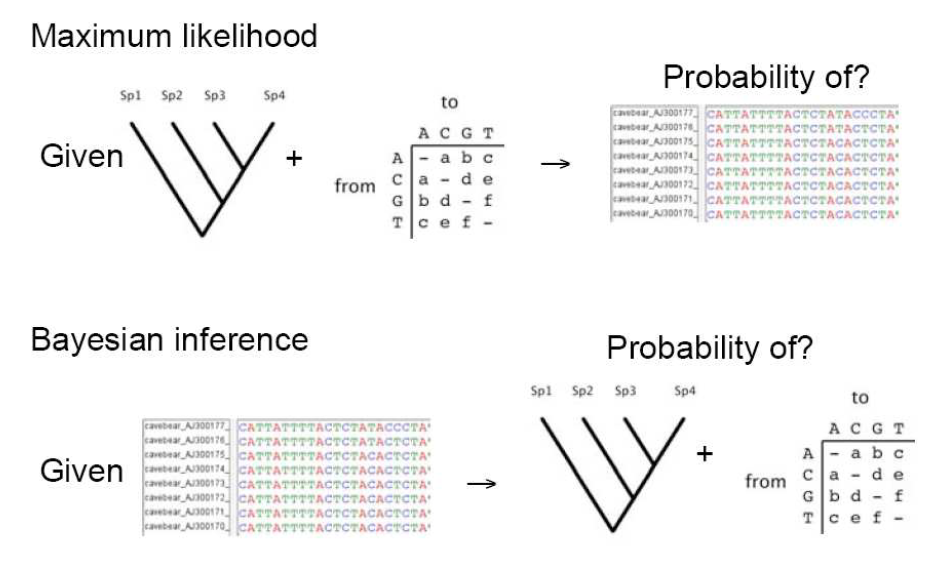
\includegraphics[height=2.5in]{MLvsBayesian.png}\\
\begin{figure}
\caption{极大似然与贝叶斯方法建树思路的比较}
\end{figure}

\end{center}

}

\frame{
\frametitle{贝叶斯方法建立进化树的MCMCMC}
1. 以任意一棵进化树$T_{i}$ 开始,计算该进化树的似然值$L_{i}$\\
2. 将进化树的参数(即拓扑结构和枝长)作随机变化,生成新的进化树$T_{j}$ ,并计算$L_{j}$\\
3. 计算两棵进化树的(似然率*先验概率)的比值$R=\frac{f(T_{j})}{f(T_{i})}$\\
4. 如果$R\geqslant1$, 则接受$T_{j}$\\
   如果$R<1$, 则在$[0,1]$之间取随机数$k$, 若$k<R$, 则保留$T_{j}$,否则拒绝接受$T_{j}$\\
5. 回到第2步\\
}


\frame{
\frametitle{MCMC在参数空间的随机游走(Random Walk)}
\begin{center}
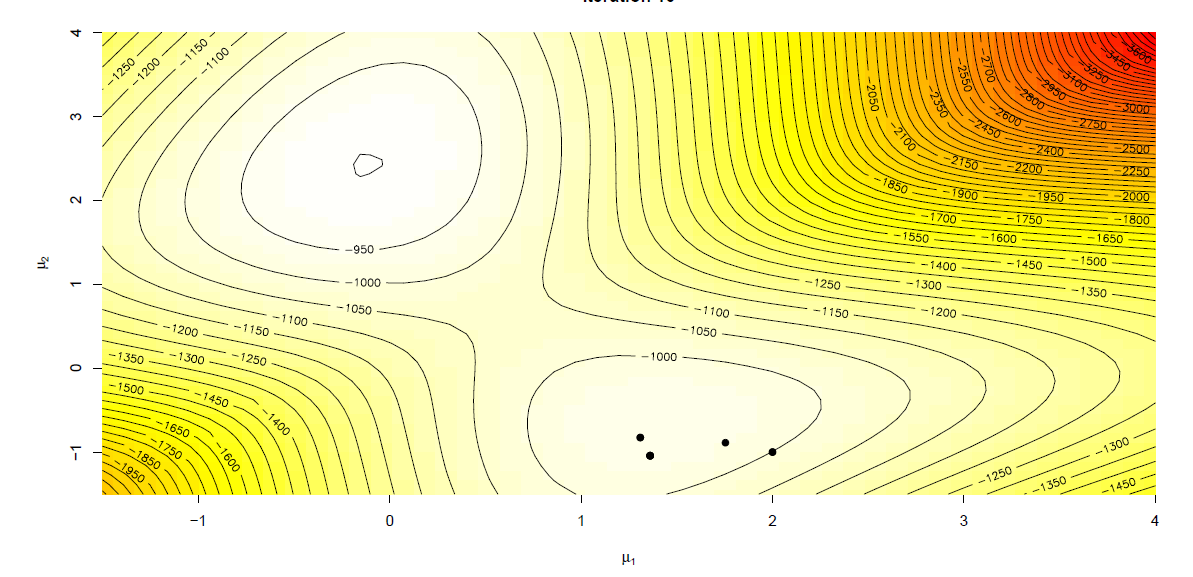
\includegraphics[height=2in]{randomwalk.png}\\

\begin{figure}
\caption{Random Walk示意图, 假设只有两个参数, 数据在两个参数组成的空间中变化。 通过MCMCMC的方法, 获得后验分布。}
\end{figure}

\end{center}
}

\frame{
\frametitle{ 冷链Cold Chain 和热链 Hot Chain}
\begin{itemize}
\item 参数随机改变的快慢程度,称为马尔科夫链的“温度”。变化越激烈,马尔科夫链越热。\\
\item 在实际情况中,往往设置若干条温度不同的马尔科夫链, 在参数空间中不断游走。\\
\item 参数变化较快的马尔科夫链,称为热链,相反则称为冷链。
\item 热链变化迅速, 便于发现概率密度更高的区域, 一旦发现概率密度更高的区域, 则冷热链交换。 \\ 
\item 冷链在概率密度更高的区域内走动, 热链则继续寻找概率密度更高的区域。\\
\item 热链用于帮助马尔科夫链收敛,冷链用于精确样本的积累。
\end{itemize}
}

\frame{
\frametitle{冷链和热链}
\begin{center}
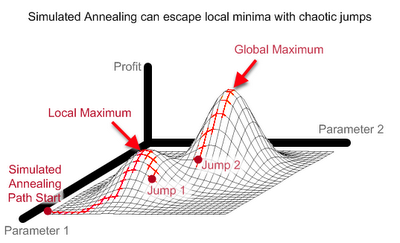
\includegraphics[height=2.5in]{mcmc.png}\\
\begin{figure}
\caption{冷链和热链示意图}
\end{figure}
\end{center}
}

\frame{
\frametitle{贝叶斯方法建树的主要软件}
\begin{itemize}
\item MrBayes:处理nexus文件,添加MrBayes命令模块。\\
\item BEAST: 处理xml文件,由Beauti生成。\\
\item PhyloBayes:用于基因组水平矩阵的计算
\end{itemize}
}


\frame{
\frametitle{贝叶斯实例}
\begin{center}
\begin{figure}
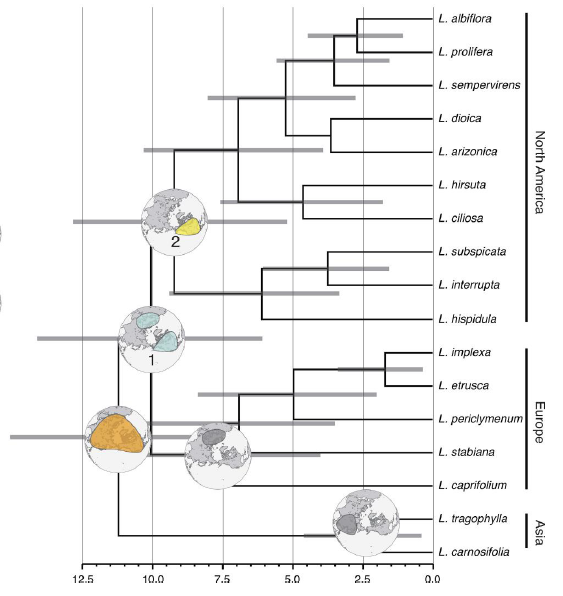
\includegraphics[height=2.5in]{BayesianTree.png}\\
\caption{北美忍冬的分化时间Smith et al. 2010}
\end{figure}
\end{center}
}

\begin{frame}
\frametitle{目录}
\section{分化时间的校对:分子钟}
\tableofcontents[currentsection] 
\end{frame}

\frame{
\frametitle{进化树枝长的意义}
\begin{itemize}
\item 距离法: 枝长表示遗传距离。\\
\item 简约法: 枝长表示变异的位点数。\\
\item 最大似然法和贝叶斯法: 枝长表示连接这段枝长的两个节点之间每个位点的期望碱基替换数。\\ % https://www.ncbi.nlm.nih.gov/pmc/articles/PMC4705742/
\end{itemize}
Chronogram: 枝长表示时间。\\
因此,一段枝长较长时, 既可能是由于分化的时间足够长, 也可能是由于碱基替换速率高, 或者两者共同的决定的。\\
分子钟校正的目的,是将遗传距离、变异的位点数等转换为chronogram。\\
}


\frame{
\frametitle{分子钟常用软件}
\begin{itemize}
\item  r8s\\
\begin{itemize}
\item 非参数速率平滑NPRS:Nonparametric rate smoothing\\
\item 似然罚分法: PL (Penalized likelihood)\\
\end{itemize}
\item BEAST 贝叶斯法,可以在建立进化树时,直接给出经过时间校正的等距树。\\
\item PATHd8,用于较大进化树的定年\\
\item ape程序包也提供几种方法, 如PL\\
\end{itemize}
个人经验:定年要用没有多分枝结构的进化树
}

\frame{
\frametitle{分子钟示意图}
\begin{center}

\begin{figure}
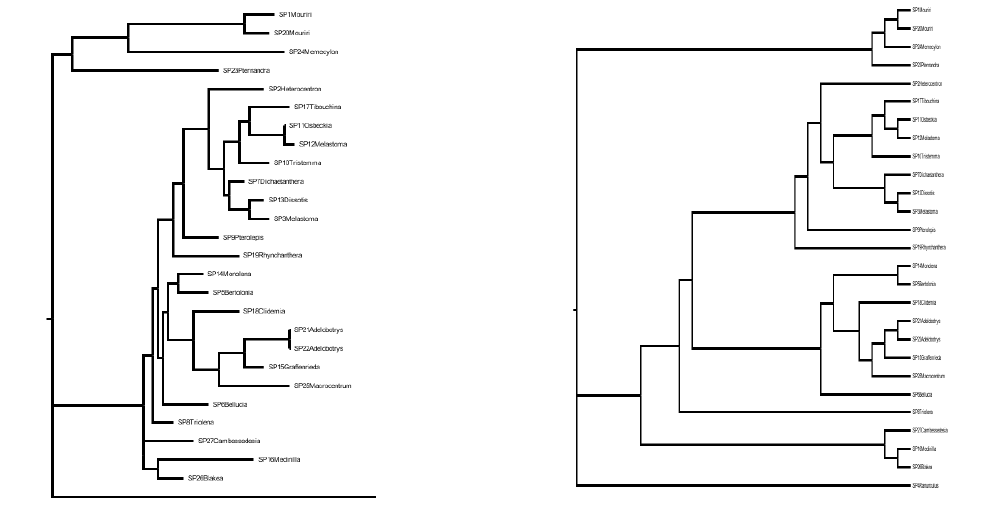
\includegraphics[height=2.2in]{NPRS.png}\\
\caption{分子钟校正前与校正后}
\end{figure}

经过分子钟校正后的进化树, 是一切系统发育多样性分析所要求输入的数据格式。
\end{center}
}

    
\begin{frame}
    \frametitle{目录}
    \section{通过植物学名建立进化树}
    \tableofcontents[currentsection]
    \end{frame}
    
    \begin{frame}
    \frametitle{通过物种名录建立进化树}
    \begin{itemize}
    \item 在DNA条形码无法获得时,人们希望通过植物名录,以现有的各大类群,如科的进化关系为基础,建立粗略的进化树。\\
    
    \item 2004年,Cam Webb博士发布了Phylomatic软件。用户输入植物名录,就可以按照指定的进化关系,生成物种水平的Newick进化树。\\ 
    
    \item 进化时间可通过Webb博士提出的BLADJ算法,并根据Wikstroem对被子植物科的分化时间进行校正。 \\
    
    \item 在科以下BLADJ算法假设,科的节点形成后, 科、属、种,各自占据三分之一的分化时间。 \\
    \end{itemize}
    
    \end{frame}
    
    \begin{frame}
    \frametitle{BLADJ算法示意图}
    \begin{center}
    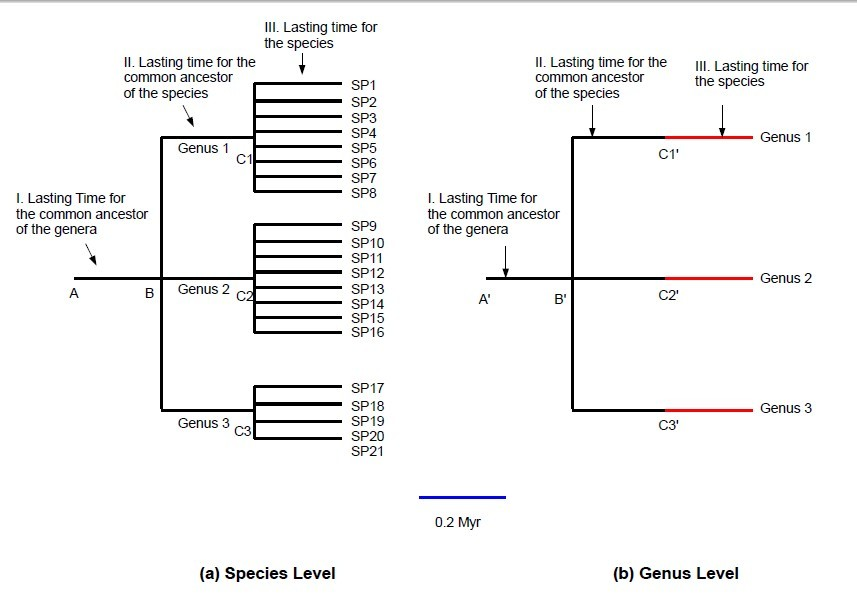
\includegraphics[height=3in]{BLADJ.png}\\
    \end{center}
    \end{frame}
    
    \begin{frame}
    \frametitle{Phylomatic的不足}
    \begin{itemize}
    \item 物种较多时,难以直接查询建树
    \item 植物之外的类群,Phylomatic未收录
    \item 不能直接输入学名,获得进化树,而是先要查询所有种的科、属、种等信息
    \end{itemize}
    \end{frame}
    
    \begin{frame}
    \frametitle{当分类单元很多:S.PhyloMaker脚本}
    \begin{center}
    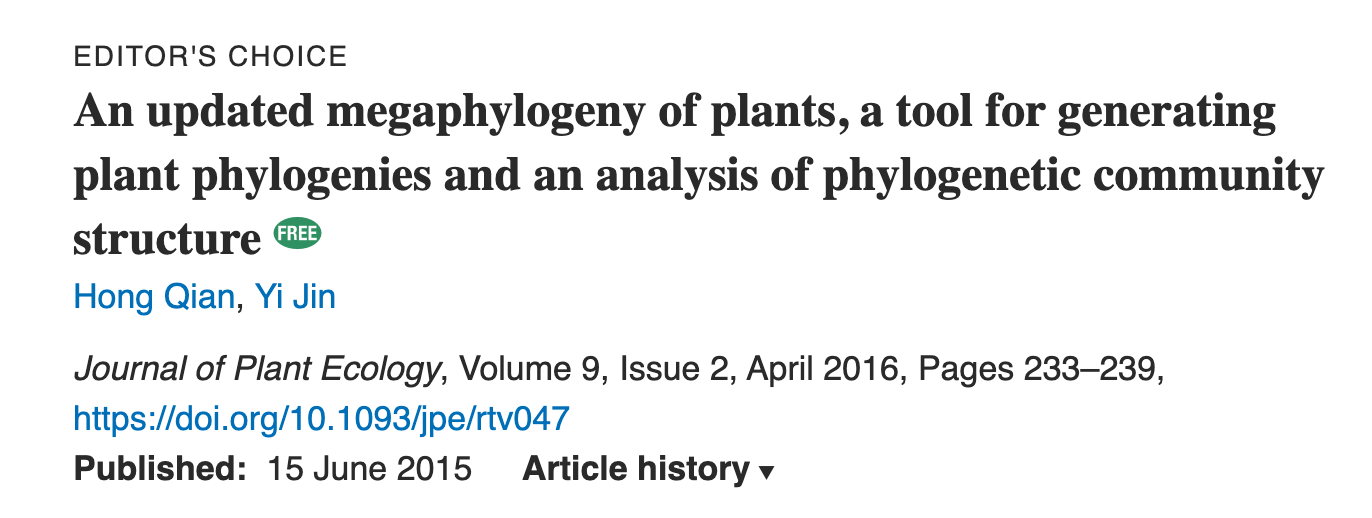
\includegraphics[height=1.8in]{sphylomaker.png}
    \end{center}
    S.PhyloMaker是一个R脚本,基于Zanne 2014的进化树,和给出的科、属、种列表,可建立包含几千种至几万分类单元的newick进化树。
    \end{frame}
    
    \begin{frame}
    \frametitle{当分类单元很多:V.PhyloMaker程序包}
    \begin{center}
    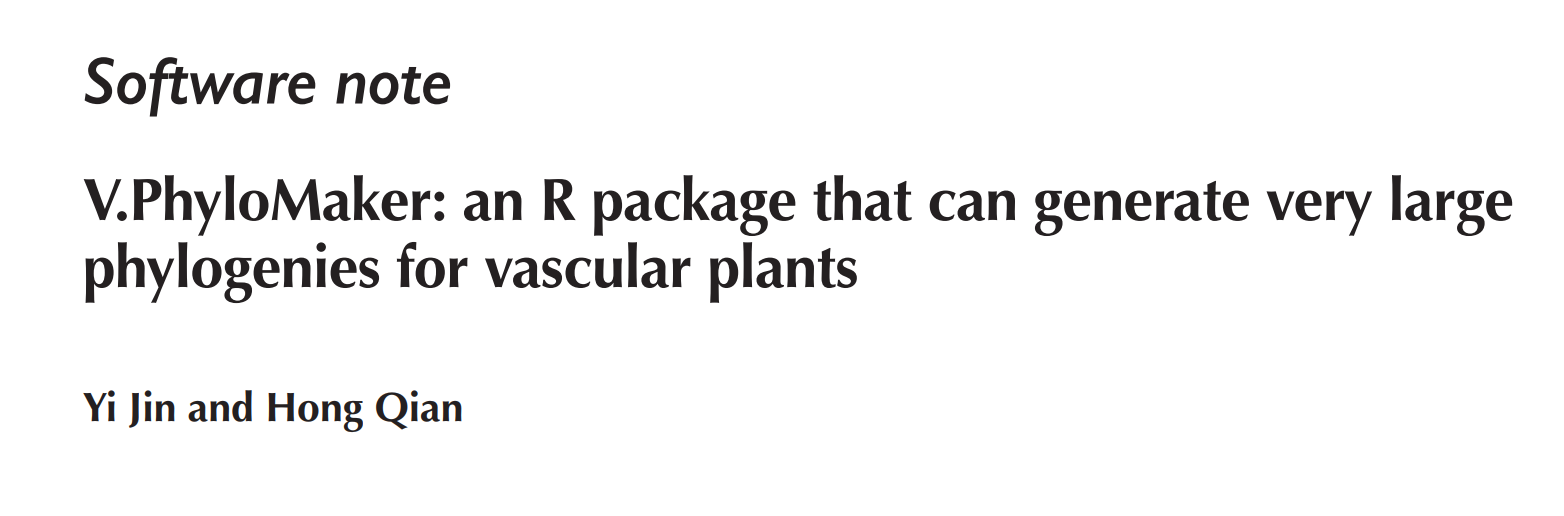
\includegraphics[height=1.6in]{v_phylomaker.png}
    \end{center}
    V.PhyloMaker基于Smith and Brown (2018) (i.e. GBOTB)的进化树,提供几种查询模式。
    \end{frame}

    \begin{frame}
    \frametitle{批量查询植物的科、属、种}
    \begin{itemize}
    \item Taxonomic Name Resolution Service \url{http://tnrs.iplantcollaborative.org/}
    \item Taxonstand R包:批量查询植物的科属
    \item taxize R包: 集成查询多种数据库
    \item plantlist R包: 批量查询科属和制作植物名录等
    \end{itemize}
    
    \end{frame}
    
    
    \begin{frame}[fragile]
    \frametitle{用plantlist批量查询科名}
     \begin{verbatim}
    # devtools::install_github("helixcn/plantlist")
    library(plantlist)
    species <- c(
    "Ranunculus japonicus",
    "Anemone udensis",
    "Ranunculus repens",
    "Ranunculus chinensis",
    "Solanum nigrum",
    "Punica sp."
    )
    col <- TPL(species)
    taxa.table(col) # 生成科属种列表
    \end{verbatim}
    \end{frame}
    

\begin{frame}
    \frametitle{目录}
    \section{系统发育多样性分析:ape、vegan和picante}
    \tableofcontents[currentsection]
    \end{frame}
    
    \begin{frame}
        \frametitle{系统发育比较分析}
        \begin{center}
        \begin{figure}
        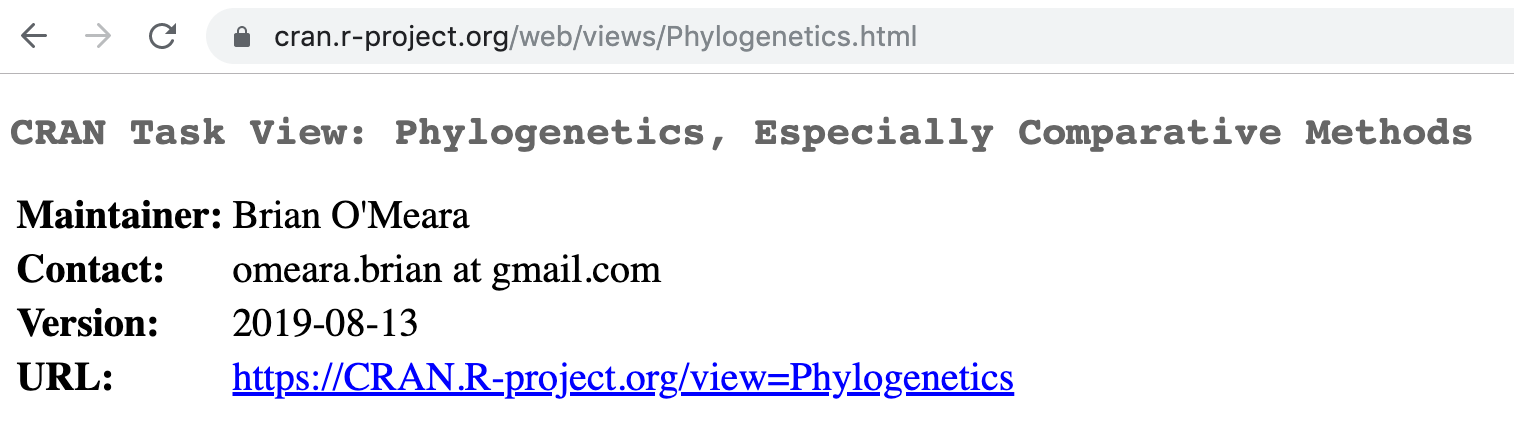
\includegraphics[height=1.6in]{view.png}\\
        \caption{CRAN Task View: Phylogenetics}
        \end{figure}
        \end{center}
        \end{frame}
        
        \begin{frame}
        \frametitle{进化树能帮我们回答哪些问题?}
        \begin{itemize}
        \item 分类单元之间的系统发育关系
        \item 物种的形成速率受什么影响?如:类群的古老程度,类群的丰富度,类群所处的纬度,类群的特殊生境
        \item 物种形成速率和灭绝速率在历史上发生过哪些变化?
        \item 物种的进化历史越独特,越应该受到保护吗?
        \item 相近的物种有相似的性状吗?有相似的习性吗?
        \end{itemize}
        \end{frame}
        
        
        \begin{frame}
        \frametitle{进化树能帮我们回答哪些问题?}
        \begin{itemize}
        \item 如果已知某一分支的性状,是否能够了解其祖先的性状?
        \item 物种的适应性是如何进化的?
        \item 已知物种的当前分布区,如何获得其祖先分布区?
        \item 群落内物种的组成是随机的,还是由于对生境的偏好造成的?
        \end{itemize}
        \end{frame}
        
        \begin{frame}
        \frametitle{系统发育比较分析的主要方向}
        \begin{itemize}
        \item  性状进化 Trait evolution
        \item  性状进化模拟 Trait Simulations
        \item  群落系统发育 Community/Microbial Ecology
        \item  祖先状态重建和气候适应性进化 Phyloclimatic Modeling
        \item  祖先分布区重建 Phylogeography/Biogeography
        \item  物种与种群的界定与模拟 Species/Population Delimitation
        \end{itemize}
        \end{frame}
    
    \begin{frame}
    \frametitle{ape程序包}
    ape是Analysis of Phylogenetics and Evolution的缩写, 作者是法国进化生物学家E. Paradis博士。
    
    ape程序包的主要功能\\
    \begin{itemize}
    \item 调整、读取和绘制进化树
    \item DNA序列的读取以及遗传距离计算
    \item 建立小型进化树
    \item 进行分子钟校正并估计进化速率
    \item 模拟生成随机进化树
    \end{itemize}
    参考: Paradis, E. (2012) Analysis of Phylogenetics and Evolution with R (Second Edition). New York: Springer. 
    \end{frame}
    
    \begin{frame}[fragile]
    \frametitle{进化树的格式:Newick进化树转换成phylo类}
    \begin{verbatim}
    # Newick进化树
    owls(((Strix_aluco:4.2,Asio_otus:4.2):3.1,Athene_noctua:
    7.3):6.3,Tyto_alba:13.5)
    
    ### 读取进化树
    tree.owls <- read.tree("ex.tre")
    \end{verbatim}
    
    显示的结果\\
    {\tt 
    Phylogenetic tree with 4 tips and 3 internal nodes.\\
    
    Tip labels:\\
    $[$1$]$ "Strix\_aluco"   "Asio\_otus" "Athene\_noctua" "Tyto\_alba"   \\ 
    
    Rooted; includes branch lengths.}\\
    
    \end{frame}
    
    \begin{frame}[fragile]
    \frametitle{进化树的格式:Newick进化树转换成List}
     \begin{verbatim}
    > str(tree.owls)
    List of 4
     $ edge   : int [1:6, 1:2] 5 6 7 7 6 5 6 7 1 2 ...
     $ Nnode  : int 3
     $ tip.label  : chr [1:4] "Strix_aluco" "Asio_otus" "Athene_noctua" "Tyto_alba"
     $ edge.length: num $[1:6]$ 6.3 3.1 4.2 4.2 7.3 13.5
     - attr(*, "class")= chr "phylo"
     - attr(*, "order")= chr "cladewise"
    \end{verbatim}
    \end{frame}
    
%%%%%%%%%% 群落数据

\begin{frame}
\frametitle{群落数据的准备和转换}
野外记录的格式
 \begin{center}
\begin{tabular}{llll} 
&plot & species &  abundance\\
1& plot1 &  sp1&3\\
2& plot1 &  sp2&6\\
3& plot1 &  sp3&1\\
4& plot1 &  sp4&2\\
5& plot1 &  sp5&1\\
6& plot2 &  sp1&8\\
7& plot2 &  sp3&   30\\
8& plot3 &  sp4&2\\
9& plot3 &  sp2&1\\
10   & plot3 &  sp6&1\\
11   & plot3 &  sp7&3\\
\end{tabular}
\end{center}
spaa::data2mat(testdata)
\end{frame}


\begin{frame}
\frametitle{转换为物种矩阵}
\begin{itemize}
\item 行表示样方, 第一列作为行名。\\
\item 列表示物种, 第一行作为物种名。\\
\item 行列交叉处表示物种的个体数, 若没有出现,则用0来表示。\\
\end{itemize}

R中物种多样性指数计算、排序、系统发育多样性分析、种间联结计算和生态位重叠分析,都使用这种矩阵。\\

\begin{center}
\begin{tabular}{llllllll} 
  & sp1 & sp2 &sp3 &sp4 & sp5 & sp6& sp7\\
  plot1   &   3 &  6  &  1 &  2 &   1 &   0&   0\\
  plot2   &   8 &  0  & 30 &  0 &   0 &   0&   0\\
  plot3   &   0 &  1  &  0 &  2 &   0 &   1&   3\\
\end{tabular}
\end{center}
\end{frame}


\begin{frame}
\frametitle{vegan程序包:群落数据分析}
Community Ecology Package: Ordination, Diversity and Dissimilarities \\
作者是芬兰生态学家Jari Oksanen.\\
\begin{itemize}
\item Alpha多样性计算: Shannon, Simpson, Pielou多样性指数等\\
\item 排序CCA、DCA、CA、NMDS\\
\item 种面积曲线\\
\item 物种多度分布曲线\\
\item 方差分解\\
\item beta多样性的计算等\\
\end{itemize}
\end{frame}

\begin{frame}[fragile]
\frametitle{alpha多样性:每个样方的多样性特征}
vegan程序包下计算多样性相关的几个指数: \\
\begin{tabular}{ll}
{\tt diversity()} &多样性计算\\
{\tt rarefy()  } &面积不等的两个群落比较时, 进行随机抽样\\
{\tt fisher.alpha()} &计算多样性\\
{\tt specnumber() } &物种数的累计\\
\end{tabular}\\


\begin{verbatim}
data(BCI)
H <- diversity(BCI)
simp <- diversity(BCI, "simpson")
invsimp <- diversity(BCI, "inv")
S <- specnumber(BCI)
J <- H/log(S)
\end{verbatim}
\end{frame}

\begin{frame}
\frametitle{beta多样性:群落之间的相似性或相异性}

{\tt{vegdist(x, method="bray", binary=FALSE, diag=FALSE, upper=FALSE, na.rm = FALSE, ...)}}\\ 
相似性指数的计算, 一般都将转换为disimmilarity 才能进行后续计算。 \\
\begin{itemize}
\item {\textbf{Jaccard}}指数: 适用于01数据,在计算beta多样性中, \\
\item {\textbf{Bray-Curtis}}指数: 适用于物种多度数据\\
\end{itemize}
\end{frame}


\begin{frame}
\frametitle{环境距离的计算:欧几里得距离}
设想二维平面直角坐标系, 有A,B两点, A坐标为$(x_1, y_1)$, B坐标为$(x_2, y_2)$\\
用dist()用来求欧几里得距离\\
\[d(A,B) = \sqrt{(x_2-x_1)^2 + (y_2-y_1)^2}\]
推广到高维:\\
\[d(p,q)=\sqrt{(q_1-p_1)^2 + (q_2-p_2)^2 + \cdots + (q_n-p_n)^2} \]
\[d(p,q)= \sqrt{\sum_{i=1}^n (q_i-p_i)^2}\]
\end{frame}


\begin{frame}[fragile]
\frametitle{欧几里得距离的计算}
\begin{verbatim}
x <- matrix(rnorm(100), nrow = 5)
dist(x)
dist(x, diag = TRUE)
dist(x, upper = TRUE)
m <- as.matrix(dist(x))
d <- as.dist(m)
\end{verbatim}
获得的距离矩阵可以进一步用于进行聚类分析等。 
\end{frame}


\begin{frame}[fragile]
\frametitle{地理距离的计算}
地球可看做近似椭球,经纬度是球面坐标,此时可用sp程序包等计算地理距离。假设A地为L1、Phi1, B地为L2,Phi2,求两地的地理距离\\
\begin{verbatim}
library(sp)
longitude <- as.numeric(c(L1, L2))
latitude  <- as.numeric(c(phi1, phi2))
cities <- c("Paris", "Washington")
location <- cbind(longitude = -longitude, latitude)
row.names(location) <- cities
location <- data.frame(location)
coordinates(location) <- ~longitude+latitude
proj4string(location) <- CRS("+proj=longlat +datum=WGS84") 
spDists(location)
\end{verbatim}

\end{frame}


\begin{frame}[fragile]
\frametitle{Mantel检验:距离矩阵之间的相关性}
两个距离矩阵的相关性不能直接用Pearson相关性来表示,而是需要用Mantel检验

{\tt ape::mantel.test(m1, m2, nperm = 999, graph = FALSE, alternative = "two.sided",  ...)}\\

示例:
\begin{verbatim}
data(varespec)
data(varechem)
veg.dist <- vegdist(varespec) # Bray-Curtis
env.dist <- vegdist(scale(varechem), "euclid")
mantel(veg.dist, env.dist)
\end{verbatim}

\end{frame}

\begin{frame}
\frametitle{beta多样性是由哪些因素决定的?}

{\color{blue}\textbf{adonis}}: Analysis of variance using distance matrices\\
 — for partitioning distance matrices among sources of variation\\
 and fitting linear models (e.g., factors, polynomial regression)\\
 to distance matrices; uses a permutation test with pseudo-F ratios.\\
{\color{blue}\textbf{mrpp}}: Multi Response Permutation Procedure and Mean Dissimilarity Matrix\\
{\color{blue}\textbf{anosim}}: Analysis of Similarities\\
{\color{blue}\textbf{MRM}}:基于Mantel test对beta多样性进行方差分解 
\end{frame}


\begin{frame}
\frametitle{系统发育信号(Phylogenetic signal)}
\begin{itemize}
\item {\color{blue}\textbf{系统发育信号(Phylogenetic signal)}}用于检验系统发育关系相近的物种是否具有相似性状。
\item Blomberg’s K(Blomberg and Garland 2002, Blomberg et al.\\ 2003, Butler and King 2004)是最常用的系统发育信号指数,K值是类群间性状差异偏离于随机过程的度量。\\
\item {\tt picante::phylosignal()}\\
\end{itemize}
\end{frame}

\begin{frame}
\frametitle{系统发育多样性}
{\color{blue}\textbf{系统发育多样性PD:Phylogenetic Diversity}}\\
\begin{itemize}
\item Faith(Faith, 1992)提出的系统发育多样性(Phylogenetic diversity,PD)给出的是某一地点所有物种在进化树上的枝长之和。\\
\item {\tt picante::pd()}\\
\end{itemize}
\end{frame}

\begin{frame}
\frametitle{为什么要提出系统发育多样性和系统发育信号?}
\begin{itemize}
\item 系统发育多样性:保护历史悠久而独特的分支类群
\item 系统发育信号:探讨性状和系统发育之间的关系
\end{itemize}
因此:系统发育多样性,常用于优先保护地的归化。系统发育信号,常用于检验近缘种,是否拥有相近的性状特征。\\

\end{frame}


\begin{frame}
\frametitle{群落系统发育的理论框架}
\begin{itemize}
\item 相似的环境,往往会选择拥有相近性状的物种,这种作用称为生境过滤作用(Environmental Filtering)。
\item 如果物种的性状越相似,系统发育关系越接近,也就是有显著的系统发育信号,那么通过分析群落内物种之间平均或者最近的系统发育距离,并将该距离和随机生成的距离相比,就可以判断生境过滤作用是否显著存在。
\item 如何实现?Cam Webb博士最早提出了基于PD的四个指数:MPD、MNTD、NRI和NTI
\end{itemize}
\end{frame}

\begin{frame}
\frametitle{MPD、MNTD、NRI和NTI}
\begin{itemize}
\item NRI和NTI是最早提出的群落系统发育指数,表示群落内物种系统发育的距离高于或者低于零模型给出的距离。\\
\item 计算群落内物种系统发育的距离常用指数有MPD和MNTD。\\
\item MPD是计算群落内物种两两之间的系统发育距离的平均值;\\
\item MNTD是寻找群落内每个物种系统发育关系最近的物种的系统发育距离,并计算所有最近物种的系统发育平均距离。 \\
MPD和MNTD和与零模型进行比较之后,分别得到NRI和NTI指数。\\
\end{itemize}
\end{frame}

\begin{frame}
\frametitle{NRI和NTI的计算}
\[NRI_{sample} = -1 \times \frac{ MPD_{sample} - MPD_{rndsample} }{sd(MPD_{rndsample})}\]\\
\[NTI_{sample} = -1 \times \frac{ MNTD_{sample} - MNTD_{rndsample} }{sd(MNTD_{rndsample})}\] \\


\begin{itemize}
\item 四个指数最早通过Phylocom软件计算,后来多通过picante软件包计算。
\item {\tt ses.mpd()} 等价于NRI
\item {\tt ses.mntd()} 等价于 NTI

\end{itemize}
\end{frame}

\begin{frame}
\frametitle{群落的零模型}
为什么要有零模型?\\
要用真实群落计算的某一指数和若干个随机化之后的群落所得指数进行比较,以观察真实值是否落在95\%的置信区间里,从而对生态学机制做出进一步的推断。
\begin{itemize}
\item 群落系统发育分析中的零模型是将群落内物种组成的关系进行随机化的一系列方法。
\item 按照中性理论,物种与物种之间是等同的,群落中物种应该是随机组合的。
\item 因此可按照一定的规则,将物种在群落内出现的方式进行随机化。
\end{itemize}

\end{frame}

\begin{frame}
\frametitle{常用的几种零模型}
群落系统发育分析中,一般通过以下四种方式进行随机化。\\
\begin{itemize}
\item {\color{blue}\textbf{Null 0}} 群落数据不变,但是物种在进化树末端随机排列。\\
\item {\color{blue}\textbf{Null 1}} 进化树不变,物种在样方中随机排列,物种从所有样方中随机选取。\\
\item {\color{blue}\textbf{Null 2}} 进化树不变,物种在样方中随机排列,物种从指定的物种库中选取。\\
\item {\color{blue}\textbf{Null 3}} 进化树不变,与此同时,物种在样方中成对的关系保持不变。这种随机化的方法称为独立交换法(Independent swap)。 \\
\end{itemize}
\end{frame}

\begin{frame}
\frametitle{系统发育beta多样性}
系统发育beta多样性是群落或地点之间系统发育距离的度量(Fine and Kembel 2010)\\
\begin{tabular}{ll}
{\color{blue}\textbf{comdist()\& comdistnn()}}&:MPD和MNTD (Webb 2000)\\
{\color{blue}\textbf{phylosor()}}&:Phylosor (Bryant et al. 2008)\\
{\color{blue}\textbf{unifrac()}}&:Unifrac(Lozupone et al. 2006)\\
{\color{blue}\textbf{rao()}}&:Rao 1982, Jost 2007, Webb et al. 2008\\
{\color{blue}\textbf{pcd()}}&:PCD (Ives and Helmus 2010)\\
\end{tabular}
\end{frame}

\begin{frame}
\frametitle{系统发育多样性研究还活跃吗?}
\begin{itemize}
\item 1 地理尺度系统发育beta多样性的成因探讨,如纬度变化,解释宏生态学的一些假说 (如 Out of Tropics假说); \\
\item 2 群落尺度内,系统发育结构、种面积曲线,系统发育多样性面积曲线和点格局分析进一步整合,以探讨群落组成的理论问题。\\ 
\item 3 群落尺度的数据和物种分布信息和适应性进一步整合,了解物种在局域尺度的适应性。\\
\end{itemize}
\end{frame}

\begin{frame}
\frametitle{系统发育多样性研究还活跃吗?II}
\begin{itemize}
\item 4 物种的功能性状数据和物种在不同尺度的分布信息,以了解物种分布和适应性的一些机理。 \\
\item 5 用功能基因组学和转录组的手段,探讨物种的适应性和分布。 \\
\item 6 借助群体遗传学,亲本分析等手段进行物种群落分布格局的研究, 进一步分析群落系统发育结构等的成因。\\
\item …… ……
\end{itemize}
\end{frame}

\frame{
\begin{center}
\LARGE {\color{blue} 
  谢~~谢!\\
  敬请批评指正!\\
} 
\end{center}
}

\end{document}
